\section{Styblinski-Tang function}
\label{sec:app:test:styblinski_tang}
  The \emph{Styblinski-Tang function} is a non-convex function used as a 
  performance test problem for optimization algorithms.
  This function is known for its complex and intricate landscape, presenting 
  numerous local minima that pose challenges to optimization algorithms.

  \begin{definition}[Styblinski-Tang function]
  \label{def:app:test:styblinski_tang}
    The Styblinski-Tang function is defined in two dimensions, with the variables \(x\) and \(y\).

    \begin{equation}
      \label{eq:app:test:styblinski_tang}
      f(\mathbf{x}) = \frac{1}{2} \sum_{i=1}^{n} 
        \left(\mathbf{x}_i^4 - 16\mathbf{x}_i^2 + 5\mathbf{x}_i\right) 
    \end{equation}
    
    where \(x\) and \(y\) are any real numbers.
  \end{definition}

  The intriguing properties of this function have made it a common benchmark in the study of algorithm performance, particularly in the field of evolutionary computation and swarm intelligence.

  \begin{figure}[ht!]
    \centering
    \begin{subfigure}[b]{0.45\textwidth}
      \centering
      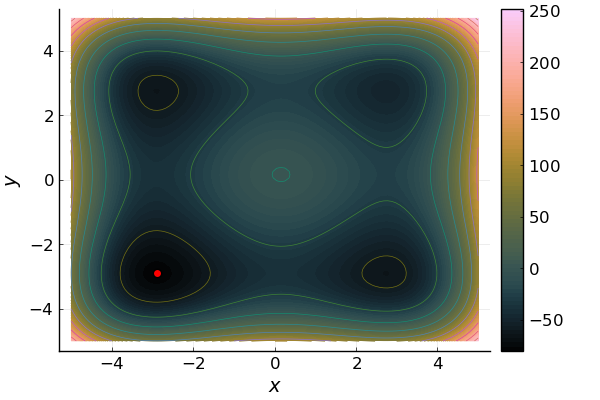
\includegraphics[width=\textwidth]{img/test_functions/styblinski_tang_contour.png}
      \caption{
        Contour plot of the Styblinski-Tang function.
        The intricate patterns show the complex landscape of the function.
        The red dot signifies the global minimum.
      }
      \label{fig:app:test:styblinski_tang:contour}
    \end{subfigure}
    \hfill
    \begin{subfigure}[b]{0.45\textwidth}
      \centering
      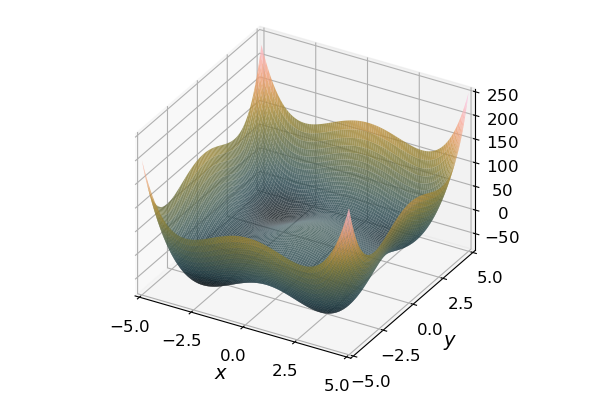
\includegraphics[width=\textwidth]{img/test_functions/styblinski_tang_surface.png}
      \caption{
        Three-dimensional surface plot of the Styblinski-Tang function.
        The plot illustrates the numerous local minima and the complex topography of the function.
      }
      \label{fig:app:test:styblinski_tang:surface}
    \end{subfigure}
    \caption{Visualizations of the Styblinski-Tang function.}
    \label{fig:app:test:styblinski_tang}
  \end{figure}